\documentclass[12pt]{article}

\usepackage{verbatim}
\usepackage{syntax}
\usepackage{listings}
\usepackage{listings}
\usepackage[T1]{fontenc}
\usepackage[polish]{babel}
\usepackage[utf8]{inputenc}
\usepackage{lmodern}
\usepackage{graphicx}
\selectlanguage{polish}
\graphicspath{ {./images/} }

\title{Algorytmika zadanie 2}
\author{
        Filip Plata \\
        Uniwersytet Warszawski
}
\date{\today}

\begin{document}
\maketitle

\section{Wstęp}

Dowód przeprowadzimy w dwóch częściach. Zaczniemy od redukcji - w czasie wielomianowym zredukujemy a) do b).

\section{Redukcja z a) do b)}

Weźmy instację problemu a) - graf dwudzielny. Tworzymy nowy graf skierowany:

W każdą krawędź grafu uv wstawaimy wierzchołek w, a krawędź uv zastępujemy poprzez uw i vw - dwie krawędzie skierowane.

Oprócz tego każdy wierzchołek grafu G rozdwajamy - na wejściowy i wyjściowy - oraz łączymy krawędzią skierowaną w stosowną stronę.

Dodajemy też wierzchołek ujście i źródło.

Źródło jest połączony do każdego wierzchołka V, a każdy wierzchołek W do ujścia.

Zauważmy, że wystarczy za zbiór A przyjąć wszystkie krawędzie wychodzące z V, kopii V (czyli pojedyńcze krawędzie pomiędzy wyjściem a wejsciem) oraz ze źródła, a za B wszystkie wchodzące do W, kopii W oraz do ujścia.

W zmienionym grafie rozwiązujemy problem b), przyjmując $k_{A} = k_{V}$ oraz $k_{B} = k_{W}$.

\subsection{Rysunek poglądowy}

Transformacja, oryginalny graf i przerobiony. Zaznaczone zbiory A i B krawędzi.

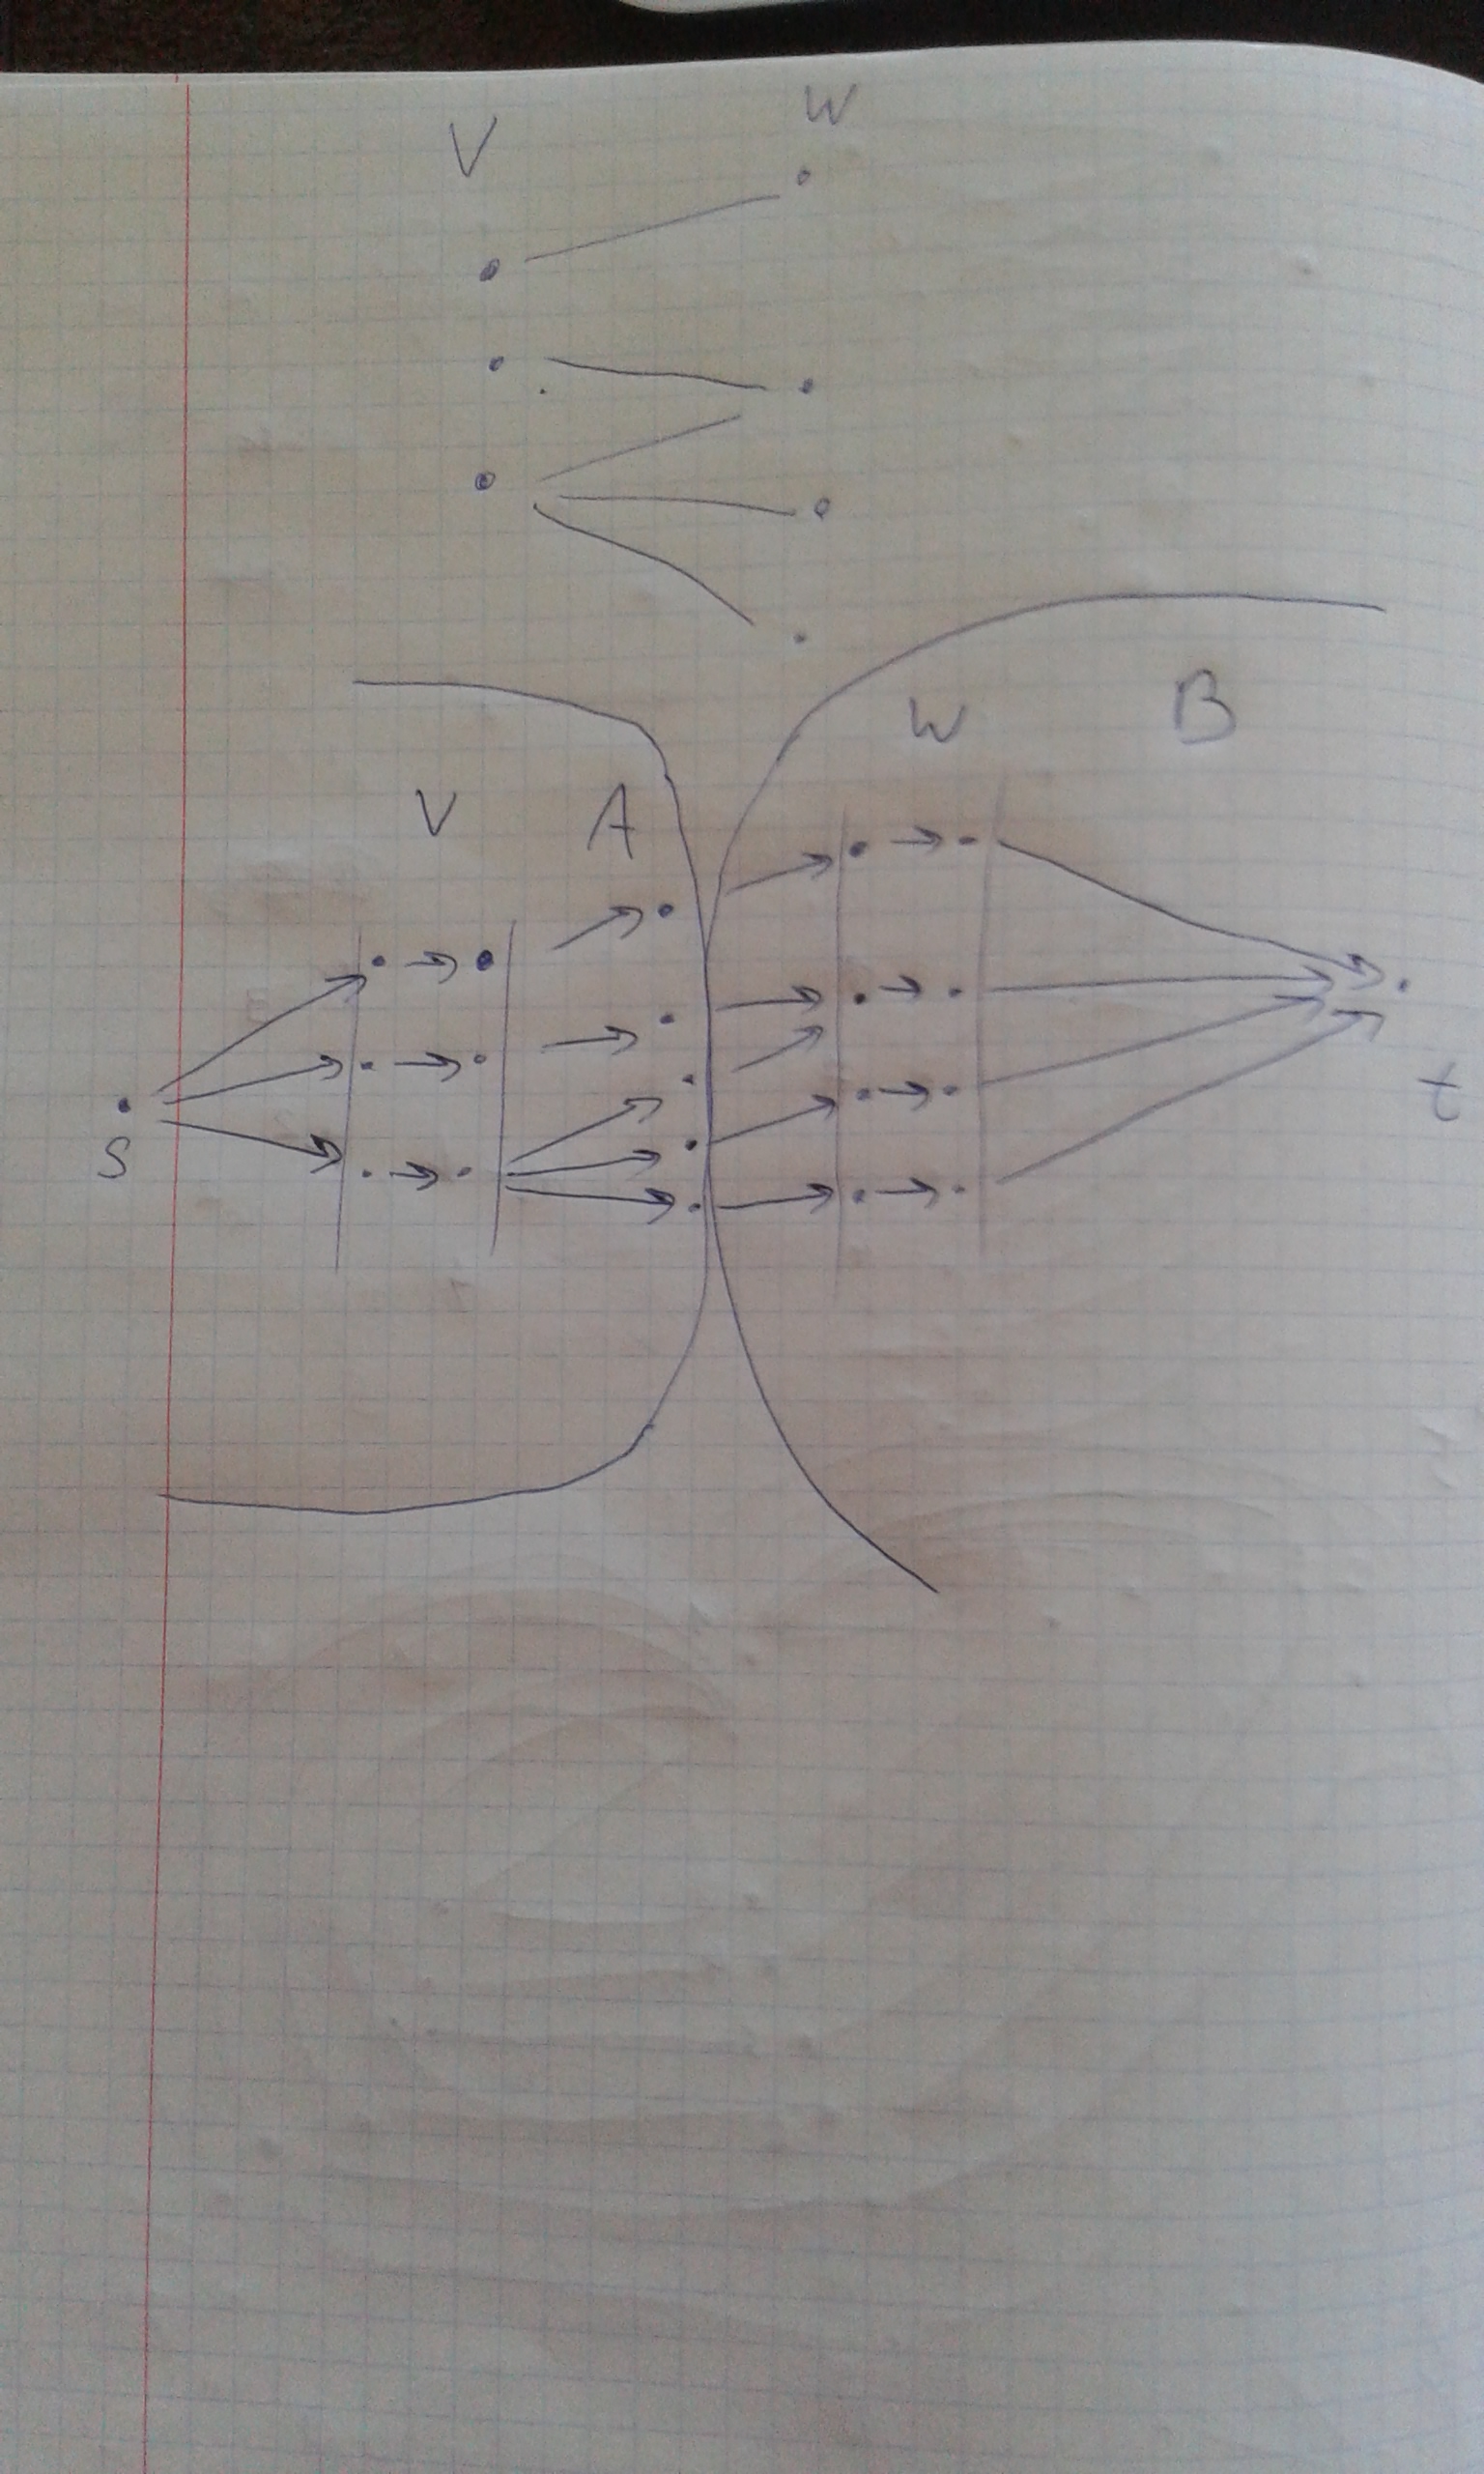
\includegraphics[scale=0.18]{transformA.png}

\subsection{Pokrycie => istnieje zbiór X krawędzi}

Jeśli istnieje pokrycie w oryginalnym grafie - do zbioru X bierzemy:

\begin{itemize}
\item dla wierzchołków z V w pokryciu - krawędzie pomiędzy ich kopią wejściową i wyjściową
\item dla W analogicznie
\end{itemize}

Wtedy nierówności zachodzą, a każda ścieżka ze źródła do ujścia przechodzi przez pewne dwie krawędzie typu wyjście-wejście i jeżeli w oryginalnym grafie dwudzielnym krawędź pomiędzy tymi wierzchołkami była pokryta, to wybraliśmy którąś z tych dwóch krawędzi - więc jedna z nich należy do X.

\subsection{Istnieje zbiór X krawędzi => Pokrycie}

Popatrzmy na krawędzie z X. Jeśli należy ona do A, jednoznacznie wyznacza ona pewien wierzchołek w oryginalnym grafie dwudzielnym, należący do V; gdyż każda taka krawędź jest jednego z trzech typów:

\begin{itemize}
\item ujście, v-in
\item v-in, v-out
\item v-in, środek-krawędzi
\end{itemize}

Dla krawędzi z B analogicznie. Wyznacza to nam zbiór wierzchołków z pokrycia w oryginalnym grafie.

Nierówności na ich liczności są oczywiście spełnione - mogliśmy wybrać tylko mniej wierzchołków.

Weźmy teraz dowolną krawędź z oryginalnego grafu dwudzielnego - vw. Weźmy w grafie po transformacji ścieżkę która przechodzi w nim po odpowiedniku (podzielonym na dwie krawędzie za pomocą wierzchołka). Ścieżka ta ma 6 krawędzi.

Jedna z krawędzi na ścieżce należy do zbioru X. Zauważmy, że na mocy konstrukcji, do pokrycia wybraliśmy jeden z wierzchołków - v albo w. Jeśli krawędź z X to jedna z trzech pierwszych - wtedy wybraliśmy v, jeśli z trzech ostatnich - wtedy dobraliśmy w.


\section{a) jest NP-hard}

Zredukujemy z problemu kliki, zgodnie z sugestią. Weźmy sobie dowolny graf G oraz liczbę k, pytamy się czy istnieje w nim klika rozmiaru k.

Transformujemy graf G do grafu dwudzielnego G'. G' składa się z dwóch zbiorów wierzchołków (części grafu dwudzielnego) - pierwsza z kopii wierzchołków, druga zawiera po jednym wierzchołku dla każdej krawędzi grafu G. Każdy wierzchołek z G' odpowiadający krawędzi otrzymuje też dwie krawędzie nieskierowane - do kopii wierzchołków które łączyła ona w nieprzetransformowanym grafie. Na wzorach:

\[ G' = (U, W, E') \]

\[ U = V \]

\[ W = \{ e' |e' \in E \} \]

\[ E' = \{ e'v | v \in V, vu \in E \lor uv \in E \} \]

Żeby rozwiązać problem kliki wystarczy w zmienionym grafie rozwiązać problem a) ze stałym $|E| - \frac{k \cdot (k-1)}{2}$ na ograniczenie wybranych wierzchołków z 'odbić' krawędzi oraz $k$ na 'odbicia' wierzchołków. Popatrzmy na to w obie strony:

\subsection{Klika => pokrycie}

Dobieramy do pokrycia wszystkie wierzchołki z kliki. Zauważmy, że wszystkie wierzchołki (krawędzie do nich wchodzące) w G' będące odbiciami krawędzi pomiędzy wierzchołkami tej kliki są pokryte. Pozostało conajwyżej $|E| - \frac{k \cdot (k-1)}{2}$ wierzchołków `krawędziowych` do pokrycia i możemy wybrać je wszystkie - pokrywając wszystkie krawędzie.

\subsection{Pokrycie => klika}

Możemy bez straty ogólności założyć, że nierówności na ilość wierzchołków pokrycia są równościami - zawsze można dobrać wierzchołki do pokrycia.

Podzielmy wierzchołki G' na cztery zbiory - obie części grafu dwudzielnego stosownie na wybrane do pokrycia i niewybrane.

Popatrzmy na krawędzie w grafie G, dla których przynajmniej jednym z końców nie jest 'odbicie' wybranego wierzchołka w G'. Zauważmy, że w pokryciu G' musieliśmy wybrać wierzchołek odpowiadający tej krawędzi - innaczej nie pokrylibyśmy którejś z dwóch krawędzi do niego wchodzących w G'.

Gdyby zatem wybrane k wierzchołków nie tworzyło kliki po powrocie z transformacji do G', musielibyśmy wybrać więcej niż $|E| - \frac{k \cdot (k-1)}{2}$ 'odbić' krawędzi w G'.
Sprzeczność.

Zatem pokrycie w G' daje istnienie kliki w G.

\end{document}
